\begin{figure}[H]
    \begin{subfigure}{\textwidth}
        \centering
        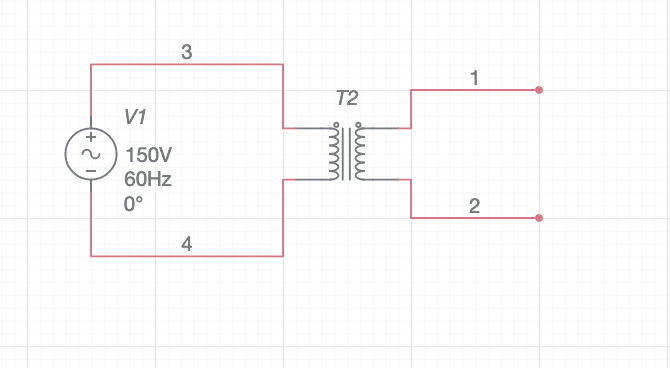
\includegraphics[width=.8\linewidth]{images/output/nol.png}
        \caption*{No load}
        \label{fig:sfig1}
    \end{subfigure}
    \caption{Circuit diagram for Transformer voltage regulation test, for no-load condition.}
\end{figure}
\begin{figure}[t]
    \begin{subfigure}{\textwidth}
        \centering
        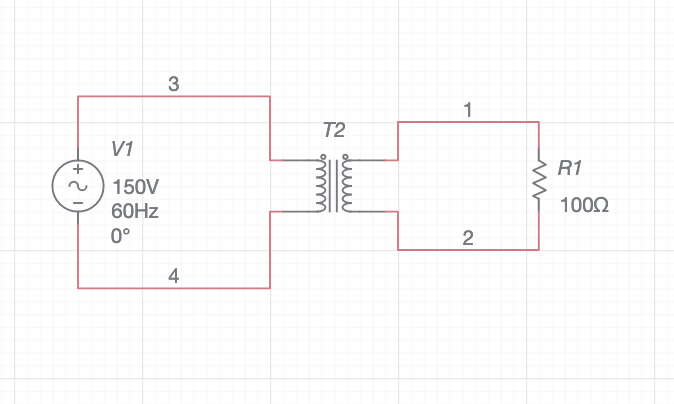
\includegraphics[width=.8\linewidth]{images/output/fl.png}
        \caption*{Resistive load}
        \label{fig:sfig2}
    \end{subfigure}
    \caption{Circuit diagram for Transformer voltage regulation test, for loaded condition.}
    \label{fig:fig}
\end{figure}
\vfill